\documentclass[conference]{IEEEtran}

% Packages
\usepackage{cite}
\usepackage{amsmath,amssymb}
\usepackage{graphicx}
\usepackage{booktabs}
\usepackage{multirow}
\usepackage{array}
\usepackage{url}
\usepackage[hidelinks]{hyperref}

\title{Ethereum Wallet Segmentation Through Layered Behavioural Validation}

\author{
\IEEEauthorblockN{Selim Balcisoy, Sena Kahya, Sude Tiras}
\IEEEauthorblockA{Faculty of Engineering and Natural Sciences\\
Sabanci University, Istanbul, Turkiye}
}

\begin{document}
\maketitle
% ============================================================
% Abstract
% ============================================================
\begin{abstract}
Public blockchains expose large-scale transaction histories, but this transparency does not automatically make wallet behaviour understandable.
This study addresses whether unsupervised Ethereum wallet segments can be interpreted as meaningful behavioural roles rather than arbitrary clustering outputs.
We propose a layered validation framework for Ethereum externally owned accounts.
After removing smart contract addresses, we construct wallet-level behavioural features, compare alternative k-means resolutions, and evaluate candidate taxonomies through feature profiles, feature-family holdouts, transaction-network null tests, monthly state transitions, two-step return behaviour, and full-population temporal signal analysis.
The analysis focuses on 2,443,868 externally owned accounts and represents daily activity through both time-domain features and frequency-domain features.
The results show that Ethereum wallet roles are interpretable and temporally structured, but they should be read as behavioural states rather than fixed real-world identities.
Across candidate resolutions, K4 provides the strongest conservative validation profile, K5 provides the highest seed stability among the compared annual resolutions and an interpretable descriptive taxonomy, and K6 provides finer-grained structure with weaker stability.
For this reason, K5 is used as the main descriptive role layer, while K4 and K6 are treated as robustness and sensitivity comparisons.
Network validation provides mixed evidence for the five-cluster taxonomy: same-role transaction concentration remains significant after Holm correction in only one of twelve monthly snapshots, although K4 and K6 show stronger network-null support.
Temporal validation shows moderate month-to-month persistence and statistically significant conditional two-step return behaviour, subject to limitations of the monthly assignment and scaling procedure.
Overall, this study contributes a reproducible framework for making Ethereum wallet behaviour readable at population scale through multiple validation layers.
\end{abstract}

\begin{IEEEkeywords}
Ethereum, wallet segmentation, behavioural clustering,
transaction networks, temporal analysis, k-means,
blockchain analytics
\end{IEEEkeywords}

% ============================================================
% 1 Introduction
% ============================================================
\section{Introduction}

Public blockchains such as Ethereum provide transaction histories at a scale that is not accessible in traditional finance.
However, having transparent data does not automatically make the system easy to understand.
A block explorer can show the activity of a single address, but rows of transaction records cannot directly explain what kinds of behavioural groups exist in the population or how those groups change over time.
Ethereum accounts differ in activity level, value flow, sending and receiving patterns, and temporal regularity.
The same account may also behave differently across different observation periods.
The main problem is therefore that large amounts of transparent transaction data are available, but the behavioural structure of the wallet population is complex and not directly interpretable from raw transactions.

One approach to this problem is wallet segmentation.
By grouping accounts with similar behavioural features, segmentation can provide a compact vocabulary for describing large-scale wallet populations.
Prior work has studied Ethereum accounts through address clustering heuristics, user profiling, graph-based deanonymization, transaction-network analysis, and temporal user representations \cite{victor2020address,beres2021blockchain,zhou2022ethident,bonifazi2022userspectra,tedge2020}.
Much of this literature is mainly concerned with entity resolution, deanonymization, identity inference, or classification into known categories.
Rather than trying to unmask wallet owners or assign accounts to pre-assumed labels, this paper asks how accounts behave and whether behavioural groups discovered by unsupervised learning are meaningful at all.

This distinction is important because unsupervised clustering will always return groups, even when the groups are weak, unstable, or difficult to interpret.
Therefore, a cluster assignment by itself does not establish a valid wallet taxonomy.
The academic question is not only whether wallets can be clustered, but whether the resulting roles are supported by additional validation evidence.
For this reason, this paper treats segmentation as a hypothesis that must be checked through multiple validation layers.

Additionally, we treat wallet behaviour as dynamic.
A wallet is not assumed to belong to a fixed role permanently.
It may be low-activity in one month, receiver-oriented in another month, and temporarily high-activity in a later period.
It may also remain in one behavioural state for a long time and then move into a different state.
This view is consistent with temporal analyses of blockchain accounts, where behavioural signatures evolve across observation windows \cite{agarwal2021temporal}.
In this paper, cluster labels are therefore interpreted as behavioural states.
They may persist, change, or recur over time, but they should not be read as verified real-world identities.

To study this problem, we use the ERC-20 Trading 2022 dataset from Harvard Dataverse \cite{somin2025erc2022,somin2025dataset}.
The initial address set contains 2,738,243 addresses.
After filtering smart contract addresses, the final analysis focuses on 2,443,868 Ethereum externally owned accounts.
We construct wallet-level aggregate features, compare alternative k-means resolutions, and evaluate candidate taxonomies through multiple validation layers.
Across the tested resolutions, K4 provides the strongest conservative validation profile, K5 provides the highest seed stability among the compared annual resolutions and an interpretable descriptive taxonomy, and K6 provides finer-grained structure with weaker stability.
For this reason, we use K5 as the main behavioural role taxonomy while treating K4 and K6 as robustness and sensitivity comparisons.
We then validate the taxonomy through transaction-network analysis, monthly transition matrices, two-step return tests, feature-family holdouts, and full-population temporal signal analysis.
The signal layer represents each wallet as a daily activity sequence and studies both direct time-domain properties and frequency-domain properties.

The main research question is:
\begin{quote}
Can Ethereum externally owned accounts be organized into behavioural states that remain meaningful across aggregate features, transaction-network evidence, and temporal activity patterns?
\end{quote}

The contribution of this work is a layered validation framework for behavioural wallet segmentation.
The framework does not claim that Ethereum naturally contains exactly five permanent wallet identities.
Instead, it shows how a candidate taxonomy can be made more defensible by testing it through feature interpretability, feature-family holdouts, shuffled-label network null models, temporal persistence, two-step return behaviour, and signal-derived activity rhythms.
Our findings suggest that Ethereum wallet behaviour is multi-layered.
Aggregate roles, transaction-network position, monthly state movement, and daily activity rhythm provide related but distinct views of the same wallet population.

% ============================================================
% 2 Motivation
% ============================================================
\section{Motivation}

Ethereum is difficult to understand directly from raw transaction data.
Although individual wallet activities can be observed through transaction records or block explorers, these tools do not explain how millions of wallets behave collectively as a population.
Relying only on manually labelled entities also provides a limited view, because most wallets do not have verified real-world labels.
Researchers, analysts, and system designers therefore need methods that can summarize large-scale wallet behaviour in a systematic and interpretable way.

Behavioural segmentation can help address this problem by converting millions of addresses into a smaller set of wallet states.
For example, analysts may want to know whether an ecosystem is dominated by low-activity wallets, persistent wallets, high-transaction wallets, high-intensity wallets, irregularly active wallets, or transitional wallets.
Such a segmentation can help describe the composition of the Ethereum ecosystem, monitor how activity patterns evolve over time, and support later applications such as anomaly detection, ecosystem monitoring, or agent-based simulation.

However, segmentation is only useful academically if the discovered groups are shown to be meaningful.
A central challenge is that wallet behaviour is dynamic.
A wallet may be inactive in one month, receiver-oriented in another month, and temporarily high-activity during a later period.
Therefore, a cluster label should not be treated as a permanent wallet identity.
Instead, wallet labels should be interpreted as behavioural states that can persist, change, or return over time.

This creates a validation problem.
In unsupervised learning, there are no ground-truth labels that directly prove whether the discovered groups are correct.
Internal metrics such as silhouette score can describe cluster compactness, but they do not prove that the clusters correspond to meaningful blockchain behaviour.
For wallet segmentation to become a research contribution, the discovered roles must be tested through additional evidence layers, including evidence that is not directly used by the clustering algorithm.

This motivates the layered design of this study.
The aggregate feature layer asks whether wallets can be grouped into interpretable roles.
The feature-holdout layer asks whether the taxonomy depends on a single feature family.
The network layer asks whether those roles align with transaction flows.
The temporal transition layer asks whether role movement is structured across months.
The two-step return layer asks whether wallets temporarily leave and return to previous states more often than expected by chance.
The temporal signal layer asks whether static roles carry distinct daily activity rhythms.
Together, these analyses evaluate the interpretability, robustness, network structure, and temporal associations of the discovered wallet roles.
The goal is not only to produce wallet clusters, but to determine what kind of evidence is needed before an unsupervised Ethereum wallet taxonomy should be trusted.

\section{Related Work}

Prior work on blockchain account analysis can be grouped into several related directions: address clustering and identity inference, Ethereum user behaviour modelling, temporal transaction-network analysis, temporal address classification, network embedding, and clustering validation.

One major direction focuses on address clustering and identity inference.
Victor studies address clustering heuristics for Ethereum and shows that on-chain behaviour can be used to link addresses under specific assumptions \cite{victor2020address}.
Similarly, B\'{e}res et al. profile and deanonymize Ethereum users by using transaction-graph information and behavioural quasi-identifiers \cite{beres2021blockchain}.
Shen et al. propose a graph-neural approach for blockchain identity inference \cite{shen2021identity}.
Zhou et al. develop Ethident, a behaviour-aware Ethereum account de-anonymization framework based on Ethereum interaction graphs \cite{zhou2022ethident}.
These studies demonstrate that Ethereum transaction behaviour contains useful information about users, addresses, and interaction patterns.
However, their main objective is usually to infer identity, ownership, address linkage, or known account categories.
Our work takes a different position.
We do not attempt to identify who controls a wallet.
Instead, we ask whether externally owned accounts can be organized into meaningful behavioural states without making real-world identity claims.

A second direction studies Ethereum users through behavioural and temporal representations.
Bonifazi et al. introduce the concept of user spectra, where Ethereum users are represented through multivariate time series of behavioural and network features \cite{bonifazi2022userspectra}.
Their work is highly relevant because it treats Ethereum behaviour as dynamic rather than static.
It shows that user activity can be represented as a temporal signal and that different users may have different behavioural profiles over time.
However, their approach focuses on supervised classification into predefined user categories.
In contrast, our study focuses on unsupervised behavioural role discovery.
Rather than starting from known labels, we first discover wallet roles from aggregate behaviour and then test whether those roles are supported by complementary validation layers.

Temporal reasoning has also been used in blockchain security and account analysis.
Agarwal et al. study malicious accounts in permissionless blockchains using temporal graph properties \cite{agarwal2021temporal}.
This work is important for our study because it shows that blockchain behaviour should be evaluated across time, not only through static snapshots.
It supports our interpretation of wallet labels as behavioural states that may persist, change, or return across observation windows.
In our work, this idea is reflected through monthly role assignments, transition matrices, and two-step return analysis.

A third direction analyzes cryptocurrency systems as evolving transaction networks.
Liang et al. study the evolutionary dynamics of Bitcoin, Ethereum, and Namecoin transaction networks using monthly network measures such as degree distribution, assortativity, clustering coefficient, and largest connected component structure \cite{liang2018evolutionary}.
Their findings show that cryptocurrency transaction networks change over time and should not be understood only as accumulated static graphs.
This motivates our use of monthly network and temporal validation.
However, their work focuses mainly on whole-network evolution.
Our study instead focuses on wallet-level behavioural segmentation and asks whether the discovered wallet roles are reflected in transaction flows.

Other studies use temporal transaction histories for address classification.
For example, functional classification approaches classify Bitcoin addresses using time-dependent balance curves and functional data analysis \cite{functionalbitcoin2023}.
This line of work is relevant because it shows that address behaviour can be represented as a temporal signal rather than only as a set of aggregate totals.
Our temporal signal layer follows a similar motivation, but differs in blockchain, task, and objective.
We study Ethereum externally owned accounts, use unsupervised clustering, and evaluate whether daily activity rhythms provide additional evidence for behavioural wallet roles.

Ethereum network embedding studies also show the importance of time and transaction value in blockchain graphs.
T-EDGE models Ethereum as a temporal weighted multidigraph and learns node embeddings that preserve transaction timing, edge multiplicity, and transferred value \cite{tedge2020}.
This supports the view that Ethereum transaction networks should be analyzed as temporal and weighted systems.
Our study differs because network information is used mainly as a validation layer for behavioural roles, rather than as the primary representation-learning objective.
In other words, we do not only ask whether a graph model can represent wallets.
We ask whether behaviourally discovered wallet roles are also visible in the transaction network.

Finally, this paper is motivated by general work on clustering validation.
Halkidi et al. emphasize that clustering results require validation because clustering algorithms can produce partitions even when the discovered groups are not meaningful \cite{halkidi2001validation}.
Liu et al. review stability estimation for unsupervised clustering and show that clustering solutions should be evaluated under perturbations such as resampling, random initialization, and changes in the input representation \cite{liu2022stability}.
These principles are central to our study.
Because wallet roles are discovered without ground-truth labels, internal clustering scores alone are not enough.
The discovered taxonomy must be tested against evidence that was not directly used to create the original clusters.

ERC-20-specific studies provide a closer network baseline.
Victor and L\"{u}ders~\cite{victor2019erc20} characterize individual
token-transfer networks and show that token-level structures can
differ from pooled-network patterns. Somin et al.~\cite{somin2025dataset}
provide the comprehensive transfer dataset underlying our 2022
analysis. These studies motivate interpreting our taxonomy within
the scope of ERC-20 transfer activity rather than all Ethereum use.

Overall, prior work shows that blockchain accounts can be studied through identity heuristics, graph structure, temporal behaviour, and representation learning.
However, fewer studies treat an unsupervised Ethereum wallet taxonomy itself as a hypothesis that requires layered validation.
This paper addresses that gap by evaluating externally owned account roles through aggregate feature profiles, transaction-network null tests, monthly temporal transitions, two-step return behaviour, and full-population temporal signal analysis.

\section{Methodology}

\begin{figure*}[t]
    \centering
    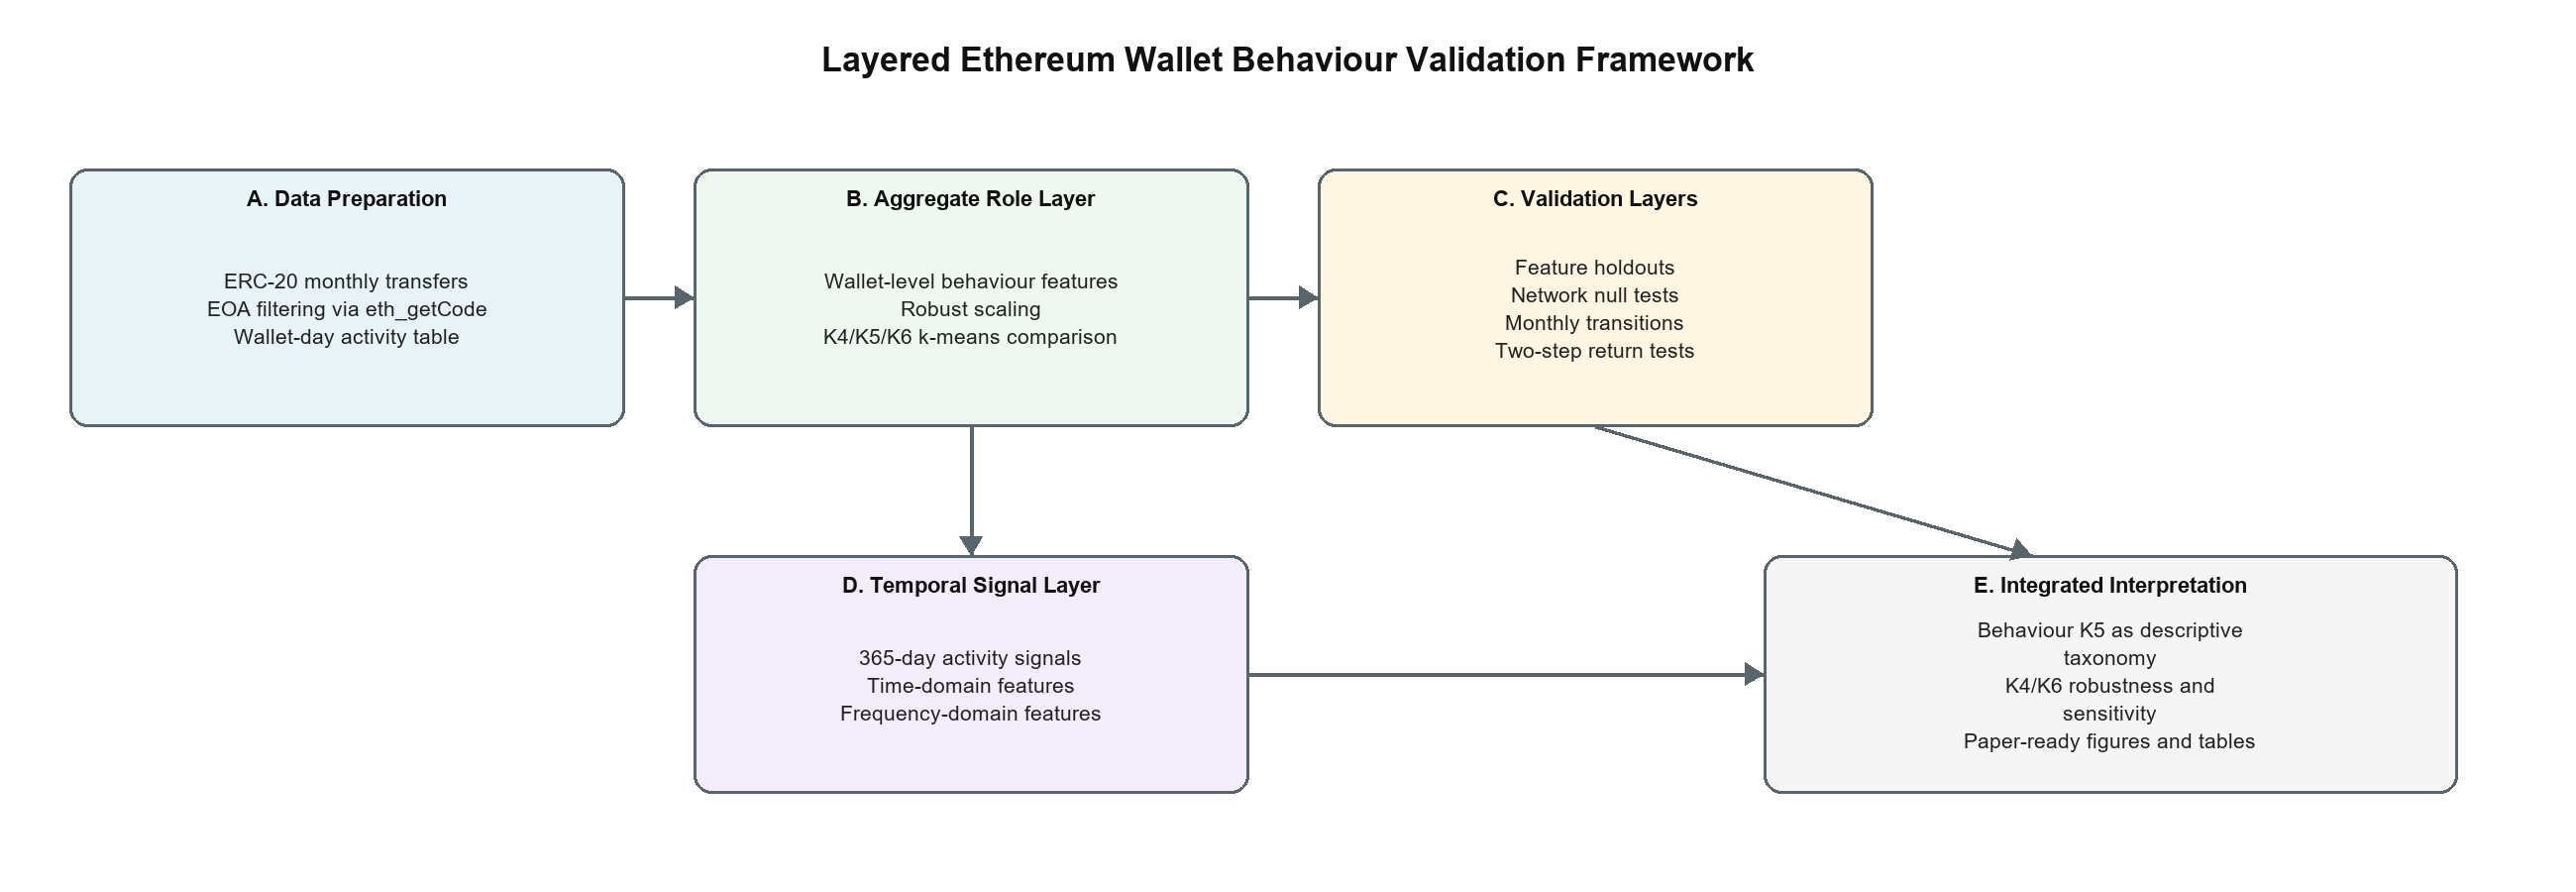
\includegraphics[width=\textwidth]{figures/ethereum_methodology.png}
    \caption{Overview of the layered Ethereum wallet behaviour
    framework. (A) ERC-20 transfer records are cleaned and
    standardized, contract addresses are removed, and a wallet-day
    activity table is constructed for externally owned accounts
    (EOAs). (B) Aggregate wallet features are transformed and
    robust-scaled before k-means clustering compares candidate
    resolutions; $k=5$ is used as the main descriptive behavioural
    taxonomy. (C) A parallel branch represents daily wallet activity
    as signals, extracts frequency-domain and time-domain features,
    and performs temporal signal clustering. (D) Feature-space,
    transaction-network, temporal-state, and cross-representation
    validation inform an integrated interpretation of aggregate
    roles and temporal activity patterns.}
    \label{fig:methodology}
\end{figure*}

\subsection{Data Preparation and EOA Filtering}

We use the 2022 subset of the Harvard Dataverse ERC-20 Trading
dataset \cite{somin2025erc2022,somin2025dataset}.
The dataset contains ERC-20 token transfer activity on Ethereum
and is part of the broader ERC-20 Trading 2015--2024 collection.
Our analysis uses the monthly 2022 transfer files, covering
January through December 2022.
The raw records are treated as ERC-20 transfer observations
represented by sender, recipient, value, and timestamp information.

For each transfer, the sender contributes an outgoing wallet
observation and the recipient contributes an incoming wallet
observation. Daily wallet records are then aggregated across
the 2022 observation window.

Contract addresses are removed before the main clustering analysis.
Address classification uses the Ethereum JSON-RPC method
\texttt{eth\_getCode} at the \texttt{latest} block.
Addresses with empty bytecode are classified as externally owned
accounts, while addresses with non-empty bytecode are classified
as contracts.

This classification reflects bytecode status at query time rather
than at the historical block of each 2022 transfer.
Contract filtering also excludes user-controlled smart-contract
wallets, such as multisignature wallets and ERC-4337 accounts.
Empty bytecode at query time does not establish that an address
was an EOA throughout 2022.

The initial mixed-address input contained 2,738,243 addresses.
The filtering step retained 2,443,868 addresses as EOAs and
excluded 294,375 addresses as contracts.
Table~\ref{tab:eoa_filtering_summary} summarizes the result.

\begin{table}[t]
    \centering
    \caption{EOA filtering summary.}
    \label{tab:eoa_filtering_summary}
    \begin{tabular}{l r}
        \toprule
        Address category & Count \\
        \midrule
        Initial mixed-address dataset & 2,738,243 \\
        Externally owned accounts retained & 2,443,868 \\
        Contract addresses removed & 294,375 \\
        \bottomrule
    \end{tabular}
\end{table}

The analysis covers ERC-20 transfer activity.
Internal execution traces and native ETH transfers are not
modelled as separate data sources.
The resulting features therefore describe ERC-20-transfer-derived
behaviour rather than all Ethereum account activity.

Token values are used as provided by the processed records.
Because ERC-20 tokens differ in units, decimals, and economic
meaning, value-flow features are interpreted as transfer-scale
indicators rather than comparable measures of economic wealth
across tokens.

The prepared wallet-day records support two analytical branches:
aggregate behavioural role discovery and temporal signal analysis.
Figure~\ref{fig:methodology} illustrates the overall workflow.

\subsection{Wallet-Level Feature Engineering}

Each wallet is represented through aggregate features describing
transaction activity, sending and receiving behaviour, value flow,
temporal persistence, volatility, and concentration.
These features capture activity intensity, temporal distribution,
directionality, and concentration of transfer activity.

Table~\ref{tab:feature_groups} summarizes the feature families.

\begin{table}[t]
    \centering
    \caption{Wallet-level behavioural feature groups.}
    \label{tab:feature_groups}
    \small
    \setlength{\tabcolsep}{3pt}
    \begin{tabular}{
        p{0.23\linewidth}
        p{0.34\linewidth}
        p{0.32\linewidth}
    }
        \toprule
        Feature group & Example features & Interpretation \\
        \midrule
        Activity intensity &
        Total transactions, mean and maximum daily transaction count &
        Overall transaction activity \\

        Temporal persistence &
        Active days, activity span, active-day ratios &
        Distribution of activity over time \\

        Directionality &
        Inflow, outflow, net flow, in/out day balance &
        Sending and receiving behaviour \\

        Value flow &
        Total, mean and maximum daily flow &
        Scale of source transfer-value aggregates \\

        Volatility &
        Daily standard deviations and coefficients of variation &
        Variability of activity \\

        Concentration &
        Transaction and flow concentration ratios &
        Concentration in a few active periods \\
        \bottomrule
    \end{tabular}
\end{table}

Before clustering, highly skewed non-negative features are
transformed using \texttt{log1p}.
Signed flow-related features use a signed logarithmic transformation.
Ratio features retain their raw form before scaling.
Each transformed feature is centred by its median and scaled
by its interquartile range.
This robust scaling reduces the influence of extreme values.

\subsection{Static Wallet Role Clustering}

We apply mini-batch k-means to the transformed and robust-scaled
EOA feature matrix, comparing $k=4$, $k=5$, and $k=6$.
Clustering uses Euclidean distance.
The reference clustering uses a fixed random seed, while
seed-stability diagnostics repeat clustering under multiple
initializations.

We select $k=5$ as the main descriptive taxonomy because it has
the highest seed stability and provides more behavioural detail
than $k=4$.
K4 provides stronger monthly network-null evidence;
K5 is therefore not claimed to be the statistically strongest
resolution.
We refer to the selected taxonomy as \emph{Behaviour K5},
retain K4 as a conservative comparison, and use K6 as a
finer-resolution sensitivity comparison.

Internal compactness and separation are assessed using
silhouette~\cite{rousseeuw1987silhouettes} and the
Davies--Bouldin index~\cite{davies1979separation}.
The comparison considers seed stability, cluster-size balance,
internal metrics, network validation, and temporal validation.
Feature-family holdouts separately assess the selected K5 taxonomy.
Table~\ref{tab:k456_comparison} summarizes the evidence.

\begin{table*}[t]
    \centering
    \caption{Comparison of EOA-only resolutions.
    Silhouette is the mean and standard deviation across five
    independent samples of 20,000 wallets with fixed annual labels;
    DB is the full-population Davies--Bouldin index.
    }
    \label{tab:k456_comparison}
    \small
    
    \begin{tabular}{c r r r c c}
        \toprule
        $k$ & Min share & Max share & Seed ARI &
        Silhouette (mean $\pm$ SD) & DB \\
        \midrule
        4 & 8.13\% & 39.56\% & 0.589 &
        $0.1632 \pm 0.0027$ & 1.6635 \\
        5 & 6.34\% & 37.78\% & 0.713 &
        $0.1611 \pm 0.0017$ & 1.6790 \\
        6 & 6.14\% & 30.50\% & 0.485 &
        $0.1678 \pm 0.0020$ & 1.6627 \\
        \bottomrule
    \end{tabular}
    
    \medskip
    
    \begin{tabular}{c c r c c c}
        \toprule
        $k$ & Network Holm & Mean obs.--null &
        Self-transition (chance) & $\kappa$ & Two-step Holm \\
        \midrule
        4 & 12/12 & 0.1096 &
        51.36\% (34.66\%) & 0.2555 & 10/10 \\
        5 & 1/12 & 0.0047 &
        50.00\% (32.32\%) & 0.2613 & 10/10 \\
        6 & 11/12 & 0.0403 &
        46.90\% (28.58\%) & 0.2566 & 10/10 \\
        \bottomrule
    \end{tabular}
    
    \smallskip

    \parbox{0.95\textwidth}{\footnotesize
    Network Holm counts significant months among twelve tests;
    two-step Holm counts significant triples among ten tests.
    Temporal quantities are conditional on the monthly
    assignment procedure.
    K4 is the conservative comparison, K5 the stable descriptive
    taxonomy, and K6 the finer-resolution sensitivity comparison.}
\end{table*}

The Behaviour K5 solution contains 2,443,868 EOAs.
Its smallest role contains 154,864 wallets (6.34\%),
and its largest contains 923,286 wallets (37.78\%).
The selected taxonomy provides a descriptive vocabulary without
highly fragmented role definitions.

\subsection{Feature Holdout Validation}

Feature-family holdout analysis tests how strongly the reference
taxonomy depends on individual feature families.
Five scenarios remove activity, value-flow, directionality,
volatility/concentration, or temporal-persistence features.

Each scenario refits mini-batch k-means with $k=5$ on the full
EOA population.
All holdouts use \texttt{MiniBatchKMeans} with random state 492,
batch size 8192, ten initializations, and a maximum of 200 iterations.

The persistence holdout removes nine features:
active days, activity span, activity density,
incoming/outgoing/both active-day counts,
and their three active-day ratios.

Candidate labels are aligned to reference labels using Hungarian
matching~\cite{kuhn1955hungarian}.
We report adjusted Rand index (ARI)~\cite{hubert1985partitions},
normalized mutual information (NMI)~\cite{vinh2010information},
exact agreement after matching, and per-cluster recovery.
ARI and NMI are computed directly between the partitions;
exact agreement and recovery use matched labels.

These experiments are robustness diagnostics.
They do not establish that the same taxonomy must appear under
every feature removal.
Because temporal-persistence features also enter annual clustering,
the relationship between annual roles and daily signal states
is not fully independent evidence.

\subsection{Transaction-Network Validation}

Network validation uses all transfers with labelled sender and
recipient addresses in each of the twelve monthly ERC-20
snapshots of 2022.
Self-transfers are removed.
Repeated transfers are retained as separate observations,
and no edge subsampling is used.

For each month and $k \in \{4,5,6\}$, we calculate the same-role
transfer ratio.
Let $E$ denote the collection of labelled transfer observations,
and let $c_i$ denote the role of wallet $i$.
Then
\begin{equation}
    R_{\mathrm{same}}
    =
    \frac{\sum_{(i,j)\in E}
    \mathbf{1}\{c_i=c_j\}}{|E|}.
\end{equation}

The null model randomly shuffles wallet labels while retaining
the transfer observations.
It tests whether same-role transfers occur more often than
expected if wallet labels were unrelated to the network.

Each test uses $B=999$ permutations with random seed 42.
The upper-tail Monte Carlo estimate is
\begin{equation}
    p =
    \frac{
        1+\sum_{b=1}^{B}
        \mathbf{1}\{R_b^{\mathrm{null}}
        \geq R^{\mathrm{obs}}\}
    }{B+1}.
\end{equation}

Holm correction~\cite{holm1979sequential} is applied across twelve monthly tests per $k$.
Fisher combined $p$-values~\cite{fisher1932methods} are also reported.
The standard chi-squared calibration assumes independent tests;
shared wallets across months may induce dependence, so the combined
value is interpreted as a supplementary summary.

For full-year role mixing, monthly transfer-count matrices
are pooled into $M$.
Expected counts under mixing with the observed outgoing and
incoming role margins are
\begin{equation}
    E_{ab}
    =
    \frac{M_{a+}M_{+b}}{M_{++}}.
\end{equation}
The mixing heatmap displays $\log_2(M_{ab}/E_{ab})$.
Directed role assortativity is calculated from the pooled matrix using the categorical mixing coefficient of Newman~\cite{newman2003mixing}.
This margin-based mixing expectation differs from the
shuffled-wallet-label null model.

Same-role network concentration is interpreted as one validation
layer rather than a necessary property of a behavioural taxonomy.
Wallets with different behaviours may interact systematically,
so weak same-role concentration does not by itself invalidate
a descriptive role taxonomy.

\subsection{Temporal Transition Analysis}

Wallet roles are treated as dynamic behavioural states.
For each month, wallet-level feature vectors are transformed
and compared with the full-year behavioural prototypes.
Each observed wallet-month is assigned to its nearest prototype.

Transitions include only wallets observed in both adjacent months.
Absence in a month is treated as missing data, not as a state.
The analysis contains 7,351,546 consecutive wallet-month
observations for each tested resolution.

For each adjacent pair, observed self-transition is the proportion
of shared wallets whose states agree.
Chance agreement is
\begin{equation}
    P_{e,t}
    =
    \sum_c p_t(c)p_{t+1}(c),
\end{equation}
where both marginals are calculated among wallets present
in that pair.

Annual observed agreement $P_o$ and expected agreement $P_e$
are weighted by pair size.
Cohen's chance-corrected agreement~\cite{cohen1960agreement} is then
\begin{equation}
    \kappa
    =
    \frac{P_o-P_e}{1-P_e}.
\end{equation}
Monthly $\kappa$ values are not averaged.

The monthly assignment procedure has two limitations.
First, counts, totals, and active-day features accumulate over
the observation window and are smaller in one month than
in the full-year representation.
Second, the monthly assignment procedure combines scaling estimated on
the mixed annual address population with EOA-only prototypes.

These mismatches may affect monthly assignments.
The reported temporal results therefore remain conditional on
the monthly assignment procedure.
Annualisation has not been applied, and chance correction
does not remove assignment bias.

\subsection{Two-Step Return Test}

For each consecutive triple $(t,t+1,t+2)$, we retain wallets
observed in all three months and then restrict the cohort to
wallets whose state changes between $t$ and $t+1$.
The observed return rate is the proportion whose state at
$t+2$ equals their state at $t$.

The null model preserves initial and middle states and permutes
final states only within middle-state strata among these eligible
first-step switchers.
It therefore preserves the selected cohort's middle-to-final
state margins while breaking wallet-specific return structure.

Each triple uses $B=999$ permutations.
Independent reproducible streams use root seed 42 together
with the resolution and triple index.
Upper-tail Monte Carlo $p$-values use the add-one estimator,
and Holm correction is applied across ten triples per $k$.

The minimum attainable Monte Carlo estimate is
$1/(999+1)=0.001$.
Reaching this resolution does not identify the true tail probability.
Pooled rates are weighted by eligible switcher observations;
wallets may occur in multiple windows.

The test asks whether the initial state carries information
about the final state beyond the middle state.
It cannot fully separate temporary excursions from stable
wallet heterogeneity or regular alternation, and does not
establish user intent.

\subsection{Full EOA Temporal Signal Analysis}

Each EOA is represented through 365-day transaction-count,
total-flow, and net-flow signals over 2022.
The signal analysis covers 2,443,868 wallets.

Time-domain features describe active days, active ratio,
total transactions, transactions per active day,
daily-count variability, maximum-to-mean transaction ratio,
active streaks, inactive gaps, active/inactive switching,
and weekly transaction-change intensity.

For transaction counts on active days, the coefficient of
variation is
\begin{equation}
    \mathrm{CV}
    =
    \frac{\sigma}{\mu},
\end{equation}
where $\sigma$ is the population standard deviation
(\texttt{ddof}=0).
A zero mean receives zero.
This feature differs from the bounded burstiness coefficient
$(\sigma-\mu)/(\sigma+\mu)$ and can exceed one.

Frequency-domain features are derived from the discrete Fourier
transform of daily transaction and flow signals.
They include dominant frequency, peak power share,
low-, medium-, and high-frequency power shares,
weekly and monthly band power shares, and spectral entropy.

These features describe the distribution of activity across
frequency components.
A dominant period near the observation window does not establish
a recurring annual cycle.

The pipeline uses streaming and disk partitioning.
Daily observations are hash-partitioned by wallet so that each
wallet's records are processed together.
Signal scaling and clustering use incremental fitting with
\texttt{MiniBatchKMeans}.

\subsection{Signal Model Selection}

Signal clustering compares $k=3$ through $k=8$ using sampled
silhouette, seed stability, cluster-size balance, and interpretability.

The selection score is
\begin{equation}
    \begin{aligned}
        S ={}& s + 0.25a \\
             &-\max(0,q_{\max}-0.75) \\
             &-\max(0,0.01-q_{\min}),
    \end{aligned}
\end{equation}
where $s$ is sampled silhouette, $a$ is mean seed ARI,
and $q_{\min}$ and $q_{\max}$ are the smallest and largest
cluster shares.
Missing silhouette is replaced by $-1$, and missing ARI by zero.
Cluster entropy is descriptive and does not enter the score.
This heuristic selects signal models rather than annual wallet roles.

The frequency-domain comparison supports $k=3$.
For time-domain features, the automatic score favours $k=3$,
but this solution places most wallets in one state.
The $k=5$ solution is retained for behavioural interpretation
because it is more balanced and more stable than the
time-domain $k=3$ solution.

Analysis scripts produce the feature, clustering, holdout,
network, transition, return, and signal outputs.
\section{Results}

\subsection{Overview of Results}

The results are organized around the layered validation logic of
the study. We compare the candidate behavioural resolutions
$k=4$, $k=5$, and $k=6$, then evaluate Behaviour K5 as the main
descriptive wallet-role taxonomy through feature-family holdouts,
transaction-network validation, monthly transitions, two-step
returns, and full-population temporal signal analysis.

No single resolution is strongest under every criterion.
Table~\ref{tab:k456_comparison} summarizes the trade-off.
K4 provides the strongest conservative network evidence. K5 has the highest seed stability and provides a richer
descriptive vocabulary. K6 offers finer structure, but lower seed
stability.

We therefore retain K5 as the primary descriptive taxonomy,
K4 as a conservative robustness reference, and K6 as a
finer-resolution sensitivity comparison. K5 is not claimed to be
statistically strongest across all validation layers.

\subsection{Static Wallet Roles}

Behaviour K5 produces five interpretable EOA roles differing in
transaction intensity, directionality, transfer scale, temporal
persistence, and volatility. These roles describe behavioural
states rather than verified real-world user identities.

Table~\ref{tab:behavior_k5_roles} summarizes the roles, and
Figure~\ref{fig:k5_profiles} shows their median robust-scaled
feature profiles. C1 is the largest role and C2 the smallest.

C2 concentrates transactions into few active days: its medians
are 3 active days, 15 transactions, and 5 transactions per active
day. C4 has the highest median active-day count among the roles:
29 active days, 65 transactions, and 2.29 transactions per active
day. Neither description implies continuous activity throughout
the year.

\begin{table*}[t]
    \centering
    \caption{Behaviour K5 wallet-role interpretation.
    Transfer-scale descriptions refer to source transfer-value
    aggregates, not comparable economic wealth across tokens.}
    \label{tab:behavior_k5_roles}
    \small
    \setlength{\tabcolsep}{4pt}
    \begin{tabular}{
        c r r
        p{0.27\textwidth}
        p{0.22\textwidth}
        p{0.16\textwidth}
    }
        \toprule
        Role & Wallets & Share &
        Behavioural description & Profile evidence & Caution \\
        \midrule

        C0 & 776,004 & 31.75\% &
        Low-transfer-scale wallets with relatively low
        transaction intensity. &
        Low-scale feature profile. &
        Interpretation remains descriptive. \\

        C1 & 923,286 & 37.78\% &
        Moderate transfer-scale wallets with larger source
        transfer-value aggregates than C0. &
        Largest role and distinct transfer-scale profile. &
        Recovery depends partly on value-flow features. \\

        C2 & 154,864 & 6.34\% &
        Concentrated high-intensity wallets: median 3 active
        days and 5 transactions per active day. &
        Distinct transaction-intensity profile. &
        High intensity does not imply persistent activity. \\

        C3 & 183,079 & 7.49\% &
        High-transaction and large-transfer-scale wallets
        with variable activity. &
        Distinct activity and transfer-scale profile. &
        Interpretation depends on model resolution. \\

        C4 & 406,635 & 16.64\% &
        Recurrent-activity wallets with a median of
        29 active days per year. &
        Highest median active-day count among K5 roles. &
        Not continuously active throughout the year. \\

        \bottomrule
    \end{tabular}
\end{table*}

\begin{figure*}[t]
    \centering
    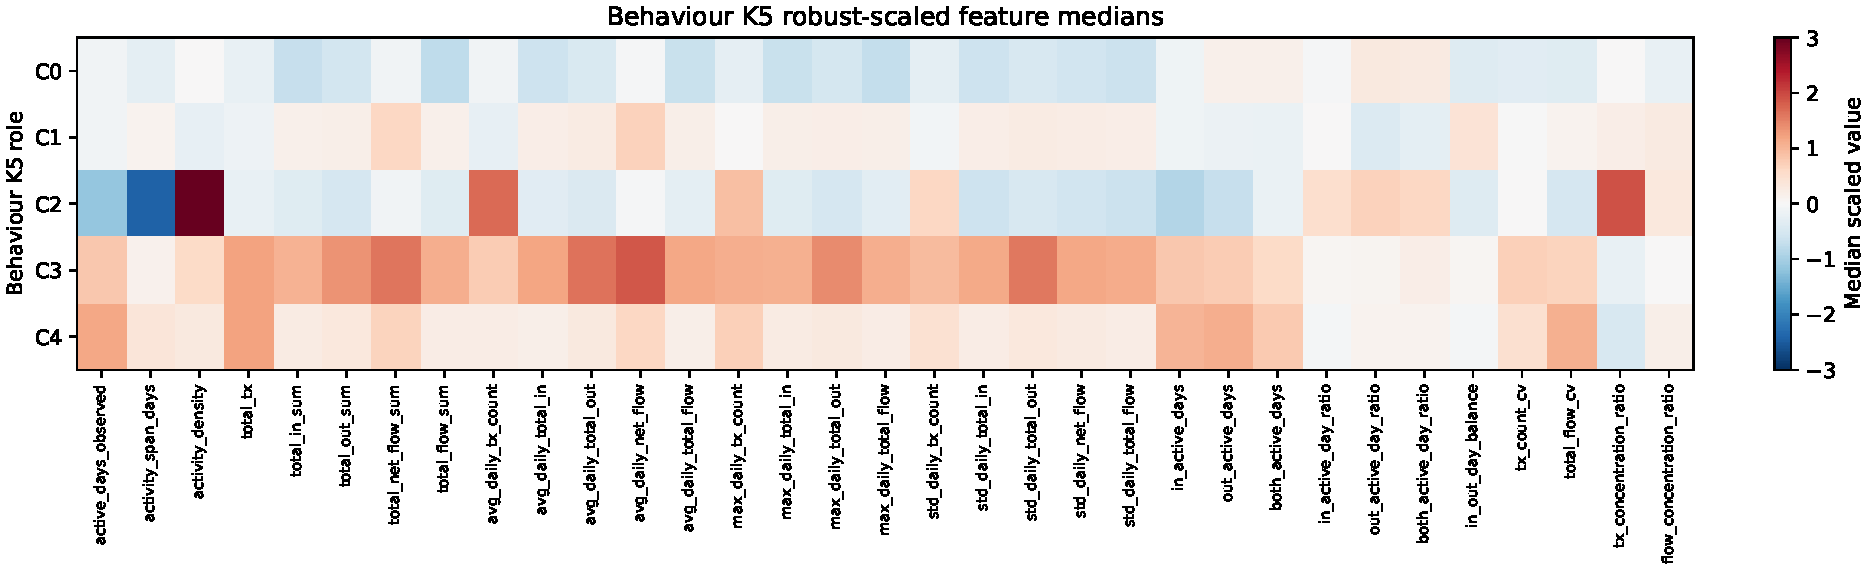
\includegraphics[width=\textwidth]
    {figures/fig_k5_profile_heatmap.pdf}
    \caption{Median robust-scaled feature profiles of Behaviour
    K5 roles. Colours show scaled feature medians; values are
    clipped at the displayed colour limits.}
    \label{fig:k5_profiles}
\end{figure*}

The five roles provide a richer behavioural vocabulary than a
coarse partition, but their interpretation must remain tied to
the observed profiles and validation results.

\subsection{Feature Holdout Robustness}

Feature-family holdouts remove one group of variables at a time,
refit mini-batch k-means with $k=5$ on the full EOA population,
and align candidate labels to the reference taxonomy.

Table~\ref{tab:feature_holdout} reports partial recovery across
feature removals. Activity, directionality,
volatility/concentration, and temporal-persistence holdouts
retain matched agreement between 61.1\% and 67.1\%.
Removing value-flow features lowers agreement to 48.1\%,
showing that transfer-scale information is important for
reproducing the reference taxonomy.

\begin{table}[t]
    \centering
    \caption{Full-population feature-family holdout validation
    for Behaviour K5. Agreement follows Hungarian label matching.}
    \label{tab:feature_holdout}
    \small
    \setlength{\tabcolsep}{3pt}
    \begin{tabular}{p{0.43\linewidth} c c c}
        \toprule
        Holdout scenario & ARI & NMI & Agreement \\
        \midrule
        Activity removed &
        0.3702 & 0.4011 & 61.1\% \\
        Value-flow removed &
        0.2391 & 0.3239 & 48.1\% \\
        Directionality removed &
        0.4616 & 0.4916 & 67.1\% \\
        Volatility/concentration removed &
        0.5032 & 0.5205 & 65.3\% \\
        Temporal-persistence removed &
        0.4126 & 0.4288 & 64.4\% \\
        \bottomrule
    \end{tabular}
\end{table}

These results indicate that the reference taxonomy is partly
recoverable without individual feature families, but is also
sensitive to the representation. The persistence holdout is
particularly relevant to the signal analysis: active days and
activity span already enter annual clustering, so associations
with time-domain states are partly expected by construction.

\subsection{Network Validation}

Figure~\ref{fig:mixing} shows full-year role-to-role mixing
relative to outgoing and incoming role margins.
Full-year K5 role assortativity is $r=-0.0243$, computed using the categorical mixing coefficient of Newman~\cite{newman2003mixing}.
This margin-based mixing expectation differs from the
shuffled-wallet-label null used for the monthly tests.
Assortativity preserves the observed outgoing and incoming role
volumes in the pooled network, whereas label shuffling preserves
the transaction graph and wallet-level role counts but allows role
transfer volumes to change. The statistics also use different
aggregation: pooled annual mixing versus an unweighted mean of
monthly differences. Consequently, slightly negative assortativity
and a slightly positive observed-minus-shuffled-null difference
are compatible.

\begin{figure}[t]
    \centering
    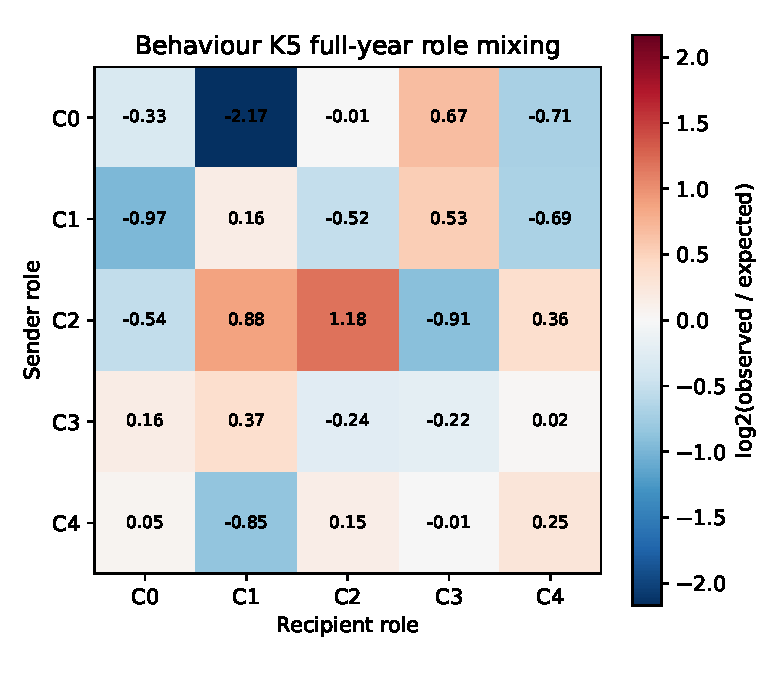
\includegraphics[width=\linewidth]
    {figures/fig2_k5_full_year_observed_expected_mixing.pdf}
    \caption{Full-year Behaviour K5 role mixing. Cells show
    $\log_2(\mathrm{observed}/\mathrm{expected})$, where expected
    counts preserve outgoing and incoming role margins.
    Positive values indicate more transfers than expected
    under this mixing baseline.}
    \label{fig:mixing}
\end{figure}

Monthly network validation uses all labelled non-self transfers
in each of the twelve 2022 snapshots and $B=999$ permutations.
For K5, three months are significant before correction,
but only one remains significant after Holm correction.

The unweighted mean of monthly observed same-role ratios is
0.2860, compared with a mean shuffled-label null ratio of 0.2813.
The mean observed-minus-null difference is 0.0047.

Figure~\ref{fig:monthly_network} compares monthly observed
and null ratios. Figure~\ref{fig:network_pvalues} shows raw
and corrected $p$-values.
Table~\ref{tab:k5_monthly_network_validation} summarizes
the results.

\begin{figure}[t]
    \centering
    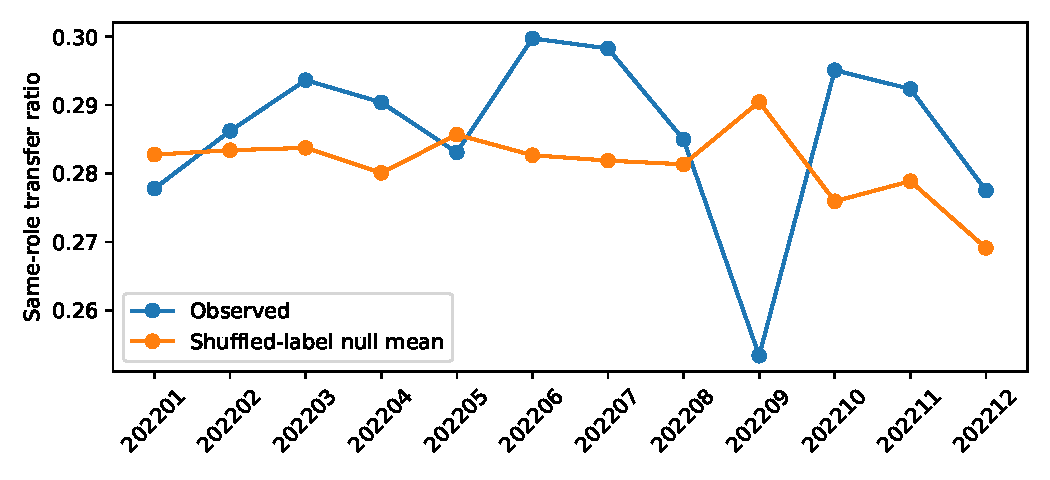
\includegraphics[width=\linewidth]
    {figures/fig3_k5_same_role_observed_vs_null.pdf}
    \caption{Monthly Behaviour K5 same-role transfer ratios
    versus the shuffled-wallet-label null mean, using all
    labelled non-self transfers and 999 permutations per month.}
    \label{fig:monthly_network}
\end{figure}

\begin{figure}[t]
    \centering
    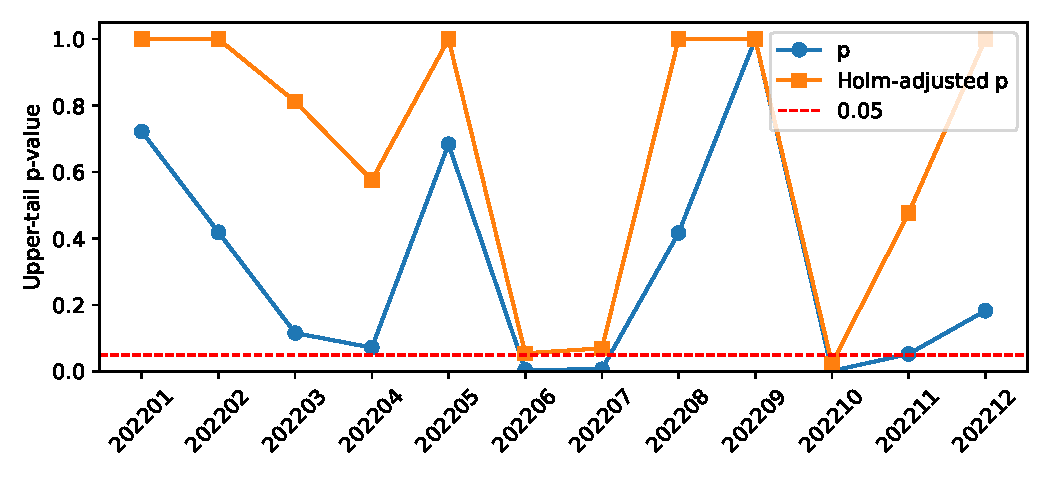
\includegraphics[width=\linewidth]
    {figures/fig4_k5_network_p_values.pdf}
    \caption{Raw and Holm-adjusted upper-tail monthly
    network-test $p$-values for Behaviour K5.
    Holm correction covers twelve months; the dashed
    line marks 0.05.}
    \label{fig:network_pvalues}
\end{figure}

\begin{table}[t]
    \centering
    \caption{Full-year Behaviour K5 transaction-network null
    validation. Mean ratios are unweighted averages across
    the twelve monthly snapshots.}
    \label{tab:k5_monthly_network_validation}
    \small
    \begin{tabular}{l r}
        \toprule
        Metric & Value \\
        \midrule
        Months tested & 12 \\
        Permutations & 999 \\
        Significant months before correction & 3 \\
        Significant months after Holm correction & 1 \\
        Mean observed same-role ratio & 0.2860 \\
        Mean shuffled-label null ratio & 0.2813 \\
        Mean observed-minus-null & 0.0047 \\
        Fisher combined $p$ & $1.8437\times10^{-4}$ \\
        \bottomrule
    \end{tabular}
\end{table}

The Fisher combined value provides evidence against the global
monthly null under its independence calibration, while only one
month survives Holm correction. Global evidence does not imply
uniform monthly significance: the evidence is concentrated in a
few months, consistent with time-varying network structure.

K5 should therefore not be interpreted as a uniformly strong
transaction-community partition. Its behavioural roles can
support analysis of interactions, but same-role concentration
is not consistently stronger than the shuffled-label null.
K4 and K6 provide stronger monthly network-null evidence.

\subsection{Temporal Transitions}

The temporal analysis contains 7,351,546 consecutive
wallet-month observations for K5.
Observed self-transition is 50.00\%, compared with 32.32\%
expected under independent consecutive states with the
pair-specific marginals. Cohen's $\kappa$ is 0.2613.

Figure~\ref{fig:self_transition_chance} compares observed
and chance-expected rates across resolutions.
Figure~\ref{fig:k5_transitions} shows K5 state-to-state
transition probabilities.
Table~\ref{tab:transition_predictiveness} reports the pooled
K5 metrics.

\begin{figure}[t]
    \centering
    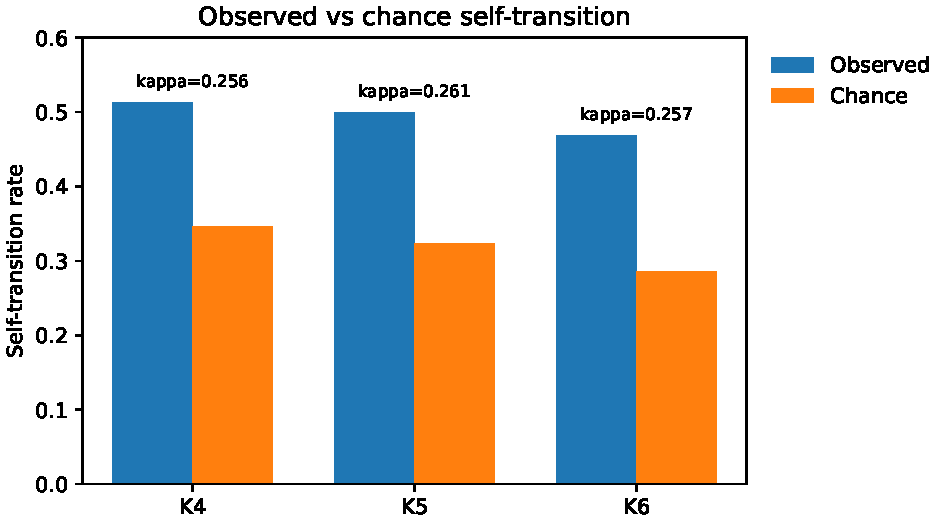
\includegraphics[width=\linewidth]
    {figures/fig_k456_self_transition_vs_chance.pdf}
    \caption{Observed and chance-expected self-transition
    rates for K4, K5 and K6. Rates use pair-size weighting;
    annotations show Cohen's $\kappa$.
    Results are conditional on the monthly
    assignment and scaling procedure.}
    \label{fig:self_transition_chance}
\end{figure}

\begin{figure}[t]
    \centering
    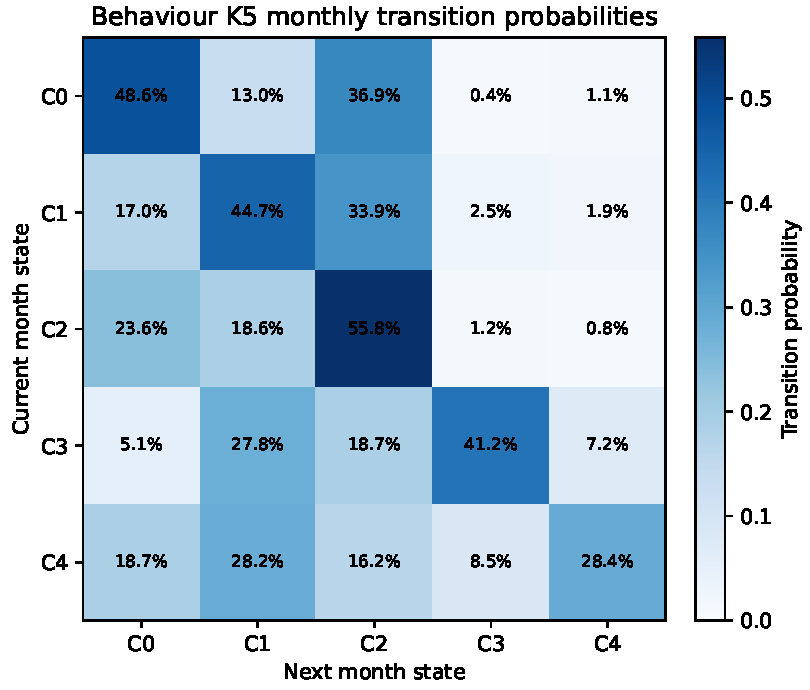
\includegraphics[width=\linewidth]
    {figures/fig_k5_transition_matrix.pdf}
    \caption{Behaviour K5 monthly transition probabilities,
    pooled over adjacent months among wallets observed in
    both months. Rows denote current states and columns
    denote next states. Results are conditional on the
    monthly assignment and scaling procedure.}
    \label{fig:k5_transitions}
\end{figure}

Knowing the current state reduces next-state entropy by 9.5\%.
The labels therefore contain measurable but non-deterministic
temporal information.

\begin{table}[t]
    \centering
    \caption{Temporal transition predictiveness of
    Behaviour K5 states.}
    \label{tab:transition_predictiveness}
    \begin{tabular}{l r}
        \toprule
        Metric & Value \\
        \midrule
        Wallet-month pairs & 7,351,546 \\
        Observed self-transition rate & 50.00\% \\
        Chance self-transition rate & 32.32\% \\
        Cohen's $\kappa$ & 0.2613 \\
        Next-state entropy & 1.783 bits \\
        Conditional entropy & 1.613 bits \\
        Normalized entropy reduction & 9.5\% \\
        \bottomrule
    \end{tabular}
\end{table}

These results remain conditional on the monthly assignment
procedure. Accumulating features are smaller in one month than
over the full year, and the monthly assignment method combines
mixed-population scaling with EOA-only prototypes.
These factors may affect state assignments; the results do
not establish causal behavioural persistence.

\subsection{Two-Step Return Behaviour}

The return test includes wallets observed in three consecutive
months that change state on the first transition.
Final states are permuted within middle-state strata among
these eligible switchers, using $B=999$ permutations.
Holm correction covers ten monthly triples.

For K5, observed return is 34.06\%, compared with a weighted
conditional-null mean of 26.24\%.
All ten triples remain significant after Holm correction.

Figure~\ref{fig:two_step_return} shows observed and
stratified-null rates for each triple.
Table~\ref{tab:two_step_return} reports the pooled
descriptive rates.

\begin{figure}[t]
    \centering
    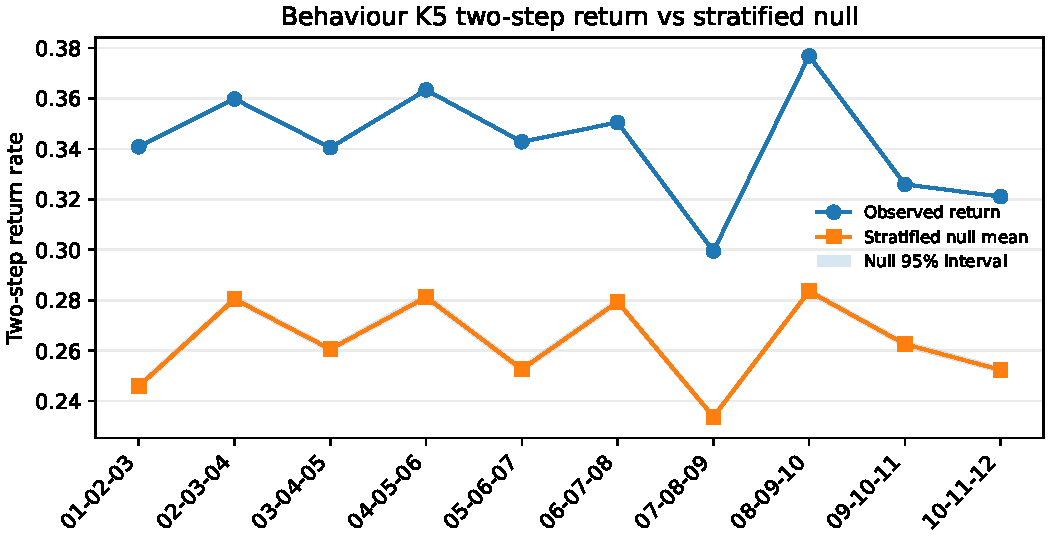
\includegraphics[width=\linewidth]
    {figures/fig_k5_two_step_return_vs_null.pdf}
    \caption{Behaviour K5 two-step return rates among
    first-step switchers observed in all three months.
    Final states are permuted within middle-state strata
    using 999 permutations. Shading shows the central
    95\% null interval, not a confidence interval for
    the observed return rate. Results are conditional
    on the monthly assignment procedure.}
    \label{fig:two_step_return}
\end{figure}

All ten raw Monte Carlo estimates reach the attainable
resolution $1/(999+1)=0.001$, with zero exceedances.
Holm-adjusted values are 0.010.
The permutation resolution does not identify the true
tail probability.

\begin{table}[t]
    \centering
    \caption{Two-step return behaviour for Behaviour K5.
    Pooled observations may include the same wallet
    in multiple monthly windows.}
    \label{tab:two_step_return}
    \begin{tabular}{l r}
        \toprule
        Metric & Value \\
        \midrule
        Eligible switcher observations & 2,352,160 \\
        Observed return rate & 34.06\% \\
        Weighted conditional-null return rate & 26.24\% \\
        Observed-minus-null & 0.0782 \\
        Permutations & 999 \\
        Significant triples before correction & 10/10 \\
        Significant triples after Holm correction & 10/10 \\
        \bottomrule
    \end{tabular}
\end{table}

The result supports conditional return structure under the
current assignment procedure. It does not establish user intent
and cannot fully separate temporary excursions from stable
wallet heterogeneity or regular alternation.

\subsection{Time-Domain Signal Results}

Daily signals provide a finer view of activity than monthly
state transitions.
Table~\ref{tab:time_domain_model_selection} compares
time-domain models.

Automatic model selection favours $k=3$, which has the
strongest silhouette score, but this solution places 76.41\%
of wallets in one cluster and has lower seed stability than
the $k=5$ solution.
We retain time-domain $k=5$ for its more balanced
descriptive state vocabulary.

\begin{table}[t]
    \centering
    \caption{Time-domain signal model-selection comparison.}
    \label{tab:time_domain_model_selection}
    \small
    \setlength{\tabcolsep}{3pt}
    \begin{tabular}{c c c c c}
        \toprule
        $k$ & Silhouette & Mean ARI &
        Max share & Selection score \\
        \midrule
        3 & 0.3011 & 0.2618 & 76.41\% & 0.3525 \\
        4 & 0.1315 & 0.3642 & 39.96\% & 0.2226 \\
        5 & 0.1638 & 0.5591 & 36.57\% & 0.3035 \\
        6 & 0.1455 & 0.3249 & 31.00\% & 0.2267 \\
        7 & 0.1418 & 0.5809 & 26.30\% & 0.2870 \\
        8 & 0.1822 & 0.4516 & 31.94\% & 0.2909 \\
        \bottomrule
    \end{tabular}
\end{table}

The five time-domain states are labelled TD0--TD4,
separately from the annual Behaviour K5 roles C0--C4.
The following profiles report arithmetic means within
each signal state.

\begin{itemize}
    \item \textbf{TD0: Intermediate variable activity}
    (15.51\%).
    Wallets average 20.35 active days and 64.02 transactions,
    with an active-day transaction-count coefficient of
    variation (CV) of 0.793.
    Their mean longest inactive gap is 131.80 days.

    \item \textbf{TD1: Sparse long-gap activity}
    (21.95\%).
    Wallets average 5.44 active days and 26.33 transactions.
    Their mean longest inactive gap is 242.74 days,
    the largest among the five states.
    The mean of wallet-specific transactions-per-active-day ratios
    is 6.86; it differs from the ratio of the state-level mean
    transaction count to mean active days.

    \item \textbf{TD2: Sparse uniform-count activity}
    (36.57\%).
    Wallets average 9.74 active days and 19.89 transactions.
    Their active-day transaction-count CV is 0.359,
    the lowest among the states, indicating relatively
    uniform counts when active rather than regular
    calendar timing.

    \item \textbf{TD3: Intermediate recurrent activity}
    (22.17\%).
    Wallets average 21.75 active days, 44.66 transactions,
    and 33.56 active/inactive switches.
    The mean longest inactive gap is 121.14 days,
    so recurrence does not imply continuous activity.

    \item \textbf{TD4: Frequent intermittent-switching activity}
    (3.81\%).
    Wallets average 93.73 active days,
    1,099.78 transactions, and 87.71 active/inactive switches,
    the highest values among the five states.
\end{itemize}

TD4's transaction-count coefficient of variation on
active days is 1.016.
This is $\sigma/\mu$, not the bounded standard burstiness
coefficient, so values above one are possible.

\subsection{Frequency-Domain Signal Results}

Frequency-domain features describe the distribution of
activity across spectral components.
Table~\ref{tab:frequency_model_selection} shows that
$k=3$ has the strongest silhouette and seed stability
among the tested frequency-domain resolutions.

\begin{table}[t]
    \centering
    \caption{Frequency-domain signal model-selection comparison.}
    \label{tab:frequency_model_selection}
    \small
    \setlength{\tabcolsep}{3pt}
    \begin{tabular}{c c c c c}
        \toprule
        $k$ & Silhouette & Mean ARI &
        Max share & Selection score \\
        \midrule
        3 & 0.1946 & 0.8317 & 52.66\% & 0.4026 \\
        4 & 0.1743 & 0.4396 & 43.04\% & 0.2842 \\
        5 & 0.1277 & 0.5361 & 34.09\% & 0.2617 \\
        6 & 0.1186 & 0.6262 & 31.60\% & 0.2751 \\
        7 & 0.1267 & 0.5173 & 31.91\% & 0.2561 \\
        8 & 0.1305 & 0.4423 & 30.89\% & 0.2360 \\
        \bottomrule
    \end{tabular}
\end{table}

The three frequency-domain states are labelled F0--F2.
Names describe spectral profiles rather than verified
periodic behaviour.
The following values are state means for the daily
transaction-count spectrum.

\begin{itemize}
    \item \textbf{F0: Distributed high-frequency activity}
    (52.66\%).
    High-frequency components contain 82.11\% of
    spectral power, compared with 5.68\% in the
    low-frequency band.
    Spectral entropy is 6.952 bits, the highest among
    the three states, and peak power share is 2.85\%,
    indicating broadly distributed power.

    \item \textbf{F1: Mixed-frequency activity}
    (40.93\%).
    High-frequency power remains dominant at 70.08\%,
    but low- and medium-frequency shares are higher
    than in F0, at 13.07\% and 16.85\%, respectively.
    Spectral entropy is 6.789 bits and peak power
    share is 4.54\%.

    \item \textbf{F2: Concentrated-activity spectrum}
    (6.41\%).
    Low-frequency power share is 36.61\% and peak
    power share is 13.99\%, both the highest among
    the states.
    Spectral entropy is 5.799 bits, the lowest among
    the three states, indicating more concentrated power.
\end{itemize}

For a 365-day observation window, the F2 profile is
consistent with activity concentrated within the year
rather than evidence of a recurring annual cycle.
High-frequency power in F0 or F1 likewise does not
establish a regular short-period cycle; sparse or
irregular daily activity can also produce broad
high-frequency power.

\subsection{Relationship Between Behaviour K5 and Signal States}

Tables~\ref{tab:k5_time_domain_bridge}
and~\ref{tab:k5_frequency_bridge} connect annual roles
to daily signal states.
Their distributions vary across K5 roles, indicating
distinct temporal signatures.

These associations are complementary evidence.
They are not fully independent validation because
activity and persistence features also enter
annual clustering.

In the time-domain analysis, 76.5\% of C2 wallets fall
in TD1, a sparse long-gap state, corresponding to
3.49-fold enrichment over its global share.

C3 is enriched in TD4: 20.3\% of its wallets belong
to that state, compared with 3.81\% globally,
giving 5.32-fold enrichment.
C4 has 3.59-fold TD4 enrichment.

\begin{table}[t]
    \centering
    \caption{Dominant time-domain subgroup within each
    Behaviour K5 role. Share is the subgroup proportion
    within the role. Active days and Switches are
    arithmetic means among wallets in that subgroup,
    not among all wallets of the role.}
    \label{tab:k5_time_domain_bridge}
    \small
    \setlength{\tabcolsep}{0pt}
    \begin{tabular*}{\linewidth}
    {@{\extracolsep{\fill}} c c c c c}
        \toprule
        K5 & TD & Share & Active days & Switches \\
        \midrule
        C0 & TD2 & 66.2\% & 9.82 & 15.45 \\
        C1 & TD2 & 33.2\% & 9.05 & 15.33 \\
        C2 & TD1 & 76.5\% & 3.30 & 3.60 \\
        C3 & TD0 & 33.5\% & 24.96 & 30.78 \\
        C4 & TD3 & 44.8\% & 32.80 & 47.49 \\
        \bottomrule
    \end{tabular*}
\end{table}

In the frequency-domain analysis, 29.2\% of C3
wallets belong to F2, giving 4.55-fold enrichment.
C4 and C2 show 1.85-fold and 2.14-fold
F2 enrichment respectively.

\begin{table}[t]
    \centering
    \caption{Concentrated-activity spectral state F2
    enrichment within Behaviour K5 roles.}
    \label{tab:k5_frequency_bridge}
    \begin{tabular}{c c c}
        \toprule
        Behaviour K5 & F2 share & F2 enrichment \\
        \midrule
        C0 & 3.8\% & 0.60$\times$ \\
        C1 & 0.5\% & 0.07$\times$ \\
        C2 & 13.7\% & 2.14$\times$ \\
        C3 & 29.2\% & 4.55$\times$ \\
        C4 & 11.8\% & 1.85$\times$ \\
        \bottomrule
    \end{tabular}
\end{table}

C3 is therefore associated with both intermittent
switching and concentrated spectral activity,
while C2 is associated with sparse long-gap behaviour.

The evidence supports a descriptive behavioural-state
taxonomy with temporal structure, rather than fixed
wallet identities or uniformly strong transaction
communities.
Temporal conclusions remain conditional on the
monthly assignment and scaling procedure,
and K4 remains the stronger conservative
network reference.

\section{Discussion}

The results support a layered interpretation of Ethereum wallet
behaviour. Aggregate clustering provides a descriptive vocabulary
of roles, while network validation shows that behavioural
similarity does not necessarily imply transaction-community
structure. For Behaviour K5, same-role transfer concentration is
significant in only one of twelve monthly networks after Holm
correction, compared with twelve months for K4 and eleven for K6.
K5 should therefore be interpreted as a descriptive behavioural
taxonomy rather than a consistently assortative network partition.

Model selection involves a trade-off between resolutions.
K4 provides stronger conservative network evidence. K5 has the highest seed
stability and offers a more detailed role vocabulary than K4.
K6 provides finer structure, but lower seed stability. These findings motivate
the use of K5 as the main descriptive taxonomy, with K4 and K6
retained as robustness and sensitivity comparisons. They do not
establish that K5 is statistically strongest across all criteria.

The role profiles also distinguish transaction intensity from
persistence. C2 concentrates transactions into few active days,
with medians of 3 active days and 5 transactions per active day.
C4 has the highest median active-day count among the five roles,
but its median of 29 days does not imply continuous activity
throughout the year. Transfer-scale differences must likewise
be interpreted cautiously: source transfer-value aggregates
across unlike ERC-20 tokens are not comparable measures of
economic wealth.

Feature holdouts show that the taxonomy is partially recoverable
under changes to the representation. Removing value-flow
features lowers matched agreement to 48.1\%, indicating that
transfer-scale information contributes substantially to the
reference partition. Removing nine temporal-persistence
features retains 64.4\% agreement, with ARI 0.4126 and NMI 0.4288.
The taxonomy therefore retains some structure without these
features, but the association between annual roles and daily
signal states should not be treated as fully independent
validation.

Temporal transitions provide evidence of persistence beyond
chance under the current state-assignment procedure.
For K5, observed self-transition is 50.00\%, compared with
32.32\% expected from the pair-specific state marginals,
giving Cohen's $\kappa=0.2613$.
Knowing the current state reduces next-state entropy by 9.5\%.
These results indicate measurable but non-deterministic
temporal structure.

The stratified two-step return test provides additional
conditional evidence. Among first-step switchers observed in
three consecutive months, K5 returns to its initial state in
34.06\% of eligible observations, compared with a weighted
conditional-null mean of 26.24\%. All ten triples remain
significant after Holm correction.
Because final states are permuted within middle-state strata,
the result indicates an association between initial and final
states beyond the selected cohort's middle-to-final margins.
It does not establish user intent or distinguish temporary
excursions fully from stable wallet heterogeneity and regular
alternation.

Both temporal analyses remain conditional on the monthly
assignment procedure. Counts, totals, and active-day features
accumulate over the observation window, making monthly values
smaller than annual values. The monthly assignment method also combines
scaling estimated on the mixed annual address population with
EOA-only prototypes. These mismatches may affect assignments;
chance correction and stratified permutations do not remove
that concern. Recomputing states under consistent population
scaling and comparable observation windows is necessary to
assess the sensitivity of the temporal findings.

Daily signal analysis provides a complementary representation.
C3 is enriched in the intermittent-switching state TD4 and
the concentrated-activity spectral state F2, while C2 is
concentrated in the sparse long-gap state TD1.
These associations show that annual roles carry different
temporal signatures. However, overlapping feature inputs
limit their interpretation as independent evidence.
Low-frequency spectral concentration indicates activity
concentrated within the observation year; it does not by itself
demonstrate a recurring annual cycle.

The scope of the taxonomy is also limited by the data and
address classification. It describes ERC-20-transfer-derived
activity of addresses classified as EOAs, rather than all
Ethereum activity. Contract filtering excludes user-controlled
smart-contract wallets, and bytecode queried at the latest
block does not establish an address's historical classification
throughout 2022.

Our central claim is that Behaviour K5 provides a useful
descriptive vocabulary whose strengths and limitations can be
examined through multiple validation layers.
The evidence supports feature-space differentiation and
conditional temporal structure, alongside weaker same-role
network concentration than the conservative K4 alternative.
Wallet roles remain behavioural descriptions rather than
verified identities, and the validation results establish
associations rather than causality.

\section{Conclusion}

This paper presents a layered validation framework for Ethereum EOA wallet segmentation.
Rather than treating clustering as the final result, we evaluate wallet roles using static feature profiles, feature-family holdouts, transaction-network structure, temporal transitions, two-step return behaviour, and full-population temporal signal analysis.

The findings show that Ethereum wallet behaviour is multi-dimensional.
Static K5 roles provide an interpretable aggregate taxonomy, while K4 and K6 show how the result changes under conservative and fine-grained resolutions.
Transaction-network analysis shows that network evidence is resolution-dependent: K4 provides the strongest conservative network support, K5 provides a richer descriptive taxonomy with weaker same-role network evidence, and K6 provides finer-grained structure with lower seed stability.
Temporal analysis shows that wallet behaviour changes in structured ways over time.
For K5, wallets show moderate chance-corrected persistence and statistically significant conditional two-step return behaviour.
Full EOA signal analysis further shows that these roles carry temporal signatures: some roles are enriched in sparse long-gap states, while others are enriched in intermittent switching and concentrated frequency-domain states.

Overall, the study demonstrates that Ethereum wallet segmentation becomes more academically defensible when clustering is combined with multiple validation layers.
The main conclusion is not that there is one permanent or natural set of wallet identities, but that behavioural wallet states can be discovered, interpreted, and evaluated through feature-space, network, temporal-transition, and temporal-signal evidence.
At the same time, the findings should be interpreted carefully.
Wallet labels are behavioural states rather than verified real-world identities, and temporal results remain conditional on the current monthly assignment and scaling procedure.

Future work can extend this framework by applying formal event-study methods, improving role labels through external metadata where appropriate, recomputing temporal transitions under a fully consistent monthly scaling procedure, and comparing the framework across multiple blockchain ecosystems.

\section*{Code and Data Availability}
All analysis code is available at \url{https://github.com/sudentrs/ethereum-wallet-behaviour-segmentation}.
The ERC-20 Trading 2022 data are available from Harvard Dataverse \cite{somin2025erc2022,somin2025dataset}.
The repository contains the analysis scripts, figure-generation scripts, and reproducibility notes used to generate the reported validation outputs.
Raw monthly transfer files and large derived label tables are not stored in the repository and should be regenerated or downloaded from the cited data source.
\begin{thebibliography}{99}

\bibitem{victor2020address}
F. Victor, ``Address clustering heuristics for Ethereum,'' in \emph{Financial Cryptography and Data Security}, LNCS, vol. 12059, 2020, pp. 617--633.

\bibitem{beres2021blockchain}
F. B\'{e}res, I. A. Seres, A. A. Bencz\'{u}r, and M. Quintyne-Collins, ``Blockchain is watching you: Profiling and deanonymizing Ethereum users,'' in \emph{2021 IEEE International Conference on Decentralized Applications and Infrastructures (DAPPS)}, 2021, pp. 69--78.

\bibitem{zhou2022ethident}
J. Zhou, C. Hu, J. Chi, J. Wu, M. Shen, and Q. Xuan, ``Behavior-aware account de-anonymization on Ethereum interaction graph,'' \emph{IEEE Transactions on Information Forensics and Security}, vol. 17, pp. 3433--3448, 2022.

\bibitem{bonifazi2022userspectra}
G. Bonifazi, E. Corradini, D. Ursino, and L. Virgili, ``Defining user spectra to classify Ethereum users based on their behavior,'' \emph{Journal of Big Data}, vol. 9, article 37, 2022.

\bibitem{tedge2020}
D. Lin, J. Wu, Q. Yuan, and Z. Zheng, ``T-EDGE: Temporal WEighted MultiDiGraph embedding for Ethereum transaction network analysis,'' \emph{Frontiers in Physics}, vol. 8, article 204, 2020.

\bibitem{agarwal2021temporal}
R. Agarwal, S. Barve, and S. K. Shukla, ``Detecting malicious accounts in permissionless blockchains using temporal graph properties,'' \emph{Applied Network Science}, vol. 6, article 9, 2021.

\bibitem{somin2025erc2022}
S. Somin, ``ERC-20 Trading 2022,'' Harvard Dataverse, 2025, doi: \href{https://doi.org/10.7910/DVN/5P82QC}{10.7910/DVN/5P82QC}.

\bibitem{somin2025dataset}
S. Somin, Y. Altshuler, and A. Pentland, ``Crypto-asset trading on top of Ethereum Blockchain comprehensive dataset,'' \emph{Scientific Data}, vol. 12, article 1407, 2025, doi: \href{https://doi.org/10.1038/s41597-025-05662-w}{10.1038/s41597-025-05662-w}.

\bibitem{shen2021identity}
J. Shen, J. Zhou, Y. Xie, S. Yu, and Q. Xuan, ``Identity inference on blockchain using graph neural network,'' in \emph{Blockchain and Trustworthy Systems}, CCIS, vol. 1490, 2021, pp. 3--17.

\bibitem{liang2018evolutionary}
J. Liang, L. Li, and D. Zeng, ``Evolutionary dynamics of cryptocurrency transaction networks: An empirical study,'' \emph{PLOS ONE}, vol. 13, no. 8, article e0202202, 2018.

\bibitem{functionalbitcoin2023}
M. Febrero-Bande, W. Gonz\'{a}lez-Manteiga, B. Prallon, and Y. F. Saporito, ``Functional classification of Bitcoin addresses,'' \emph{Computational Statistics \& Data Analysis}, vol. 181, article 107687, 2023.

\bibitem{halkidi2001validation}
M. Halkidi, Y. Batistakis, and M. Vazirgiannis, ``On clustering validation techniques,'' \emph{Journal of Intelligent Information Systems}, vol. 17, no. 2--3, pp. 107--145, 2001.

\bibitem{liu2022stability}
T. Liu, H. Yu, and R. H. Blair, ``Stability estimation for unsupervised clustering: A review,'' \emph{WIREs Computational Statistics}, vol. 14, no. 6, article e1575, 2022.

\bibitem{victor2019erc20}
F. Victor and B. K. L\"{u}ders, ``Measuring Ethereum-Based ERC20 Token Networks,'' in \emph{Financial Cryptography and Data Security}, LNCS, vol. 11598, 2019, pp. 113--129, doi: \href{https://doi.org/10.1007/978-3-030-32101-7_8}{\nolinkurl{10.1007/978-3-030-32101-7_8}}.

\bibitem{rousseeuw1987silhouettes}
P. J. Rousseeuw, ``Silhouettes: A graphical aid to the interpretation and validation of cluster analysis,'' \emph{Journal of Computational and Applied Mathematics}, vol. 20, pp. 53--65, 1987, doi: \href{https://doi.org/10.1016/0377-0427(87)90125-7}{10.1016/0377-0427(87)90125-7}.

\bibitem{davies1979separation}
D. L. Davies and D. W. Bouldin, ``A cluster separation measure,'' \emph{IEEE Transactions on Pattern Analysis and Machine Intelligence}, vol. PAMI-1, no. 2, pp. 224--227, 1979, doi: \href{https://doi.org/10.1109/TPAMI.1979.4766909}{10.1109/TPAMI.1979.4766909}.

\bibitem{kuhn1955hungarian}
H. W. Kuhn, ``The Hungarian method for the assignment problem,'' \emph{Naval Research Logistics Quarterly}, vol. 2, no. 1--2, pp. 83--97, 1955, doi: \href{https://doi.org/10.1002/nav.3800020109}{10.1002/nav.3800020109}.

\bibitem{hubert1985partitions}
L. Hubert and P. Arabie, ``Comparing partitions,'' \emph{Journal of Classification}, vol. 2, pp. 193--218, 1985, doi: \href{https://doi.org/10.1007/BF01908075}{10.1007/BF01908075}.

\bibitem{vinh2010information}
N. X. Vinh, J. Epps, and J. Bailey, ``Information theoretic measures for clusterings comparison: Variants, properties, normalization and correction for chance,'' \emph{Journal of Machine Learning Research}, vol. 11, pp. 2837--2854, 2010. [Online]. Available: \url{https://jmlr.org/papers/v11/vinh10a.html}

\bibitem{holm1979sequential}
S. Holm, ``A simple sequentially rejective multiple test procedure,'' \emph{Scandinavian Journal of Statistics}, vol. 6, no. 2, pp. 65--70, 1979. [Online]. Available: \url{https://www.jstor.org/stable/4615733}

\bibitem{fisher1932methods}
R. A. Fisher, \emph{Statistical Methods for Research Workers}, 4th ed. Edinburgh: Oliver and Boyd, 1932.

\bibitem{newman2003mixing}
M. E. J. Newman, ``Mixing patterns in networks,'' \emph{Physical Review E}, vol. 67, article 026126, 2003, doi: \href{https://doi.org/10.1103/PhysRevE.67.026126}{10.1103/PhysRevE.67.026126}.

\bibitem{cohen1960agreement}
J. Cohen, ``A coefficient of agreement for nominal scales,'' \emph{Educational and Psychological Measurement}, vol. 20, no. 1, pp. 37--46, 1960, doi: \href{https://doi.org/10.1177/001316446002000104}{10.1177/001316446002000104}.

\end{thebibliography}

\end{document}


